
\documentclass[preprint,12pt]{elsarticle}

\usepackage[T1]{fontenc}
\usepackage{lmodern}
\usepackage{amsmath,amssymb}
\usepackage{booktabs,array,graphicx,xcolor,tabularx}
\usepackage{microtype}
\usepackage{xspace}
\usepackage{tikz}
\usetikzlibrary{positioning,arrows.meta,fit,calc}
\usepackage[hidelinks]{hyperref}
\usepackage{url}
\Urlmuskip=0mu plus 2mu\relax
\def\UrlBreaks{\do\/\do\-\do\.}
\usepackage[capitalise,nameinlink]{cleveref}
\usepackage{caption}
\usepackage[section]{placeins}
\captionsetup{font=small,labelfont=bf}
\setlength{\emergencystretch}{2em}
\renewcommand{\topfraction}{0.9}\renewcommand{\textfraction}{0.08}\renewcommand{\floatpagefraction}{0.7}

\newcommand{\ms}{\,ms\xspace}
\newcommand{\KiB}{\,KiB\xspace}
\newcommand{\Mbits}{\,Mbit/s\xspace}
\newcommand{\cpu}{\mathrm{cpu}}

\usepackage{xr-hyper}
%\externaldocument[M-]{main}
\makeatletter
\newcommand*{\addFileDependency}[1]{%
  \typeout{(#1)}
  \@addtofilelist{#1}
  \IfFileExists{#1}{}{\typeout{No file #1.}}
}
\makeatother

\newcommand*{\myexternaldocument}[1]{%
  \externaldocument[M-]{#1}%
  \addFileDependency{#1.tex}%
  \addFileDependency{#1.aux}%
}
\myexternaldocument{main} % Thay thế cho lệnh \externaldocument thuần túy





\journal{Computers \& Security}
\hypersetup{pdfauthor={Trong-Hieu Dinh, Trong-Minh Hoang}}

\begin{document}
\begin{frontmatter}
\title{Supplementary Material for ``Modeling the Transport-Layer Latency Overhead of Post-Quantum Authentication in Financial Messaging''}
\author{Trong-Hieu DINH}
\author{Trong-Minh HOANG}
\end{frontmatter}

\noindent This document contains Appendices SA--SF of the article. Section, table, figure and equation numbers without a letter prefix refer to the article.
\appendix
\counterwithin*{table}{section}\counterwithin*{figure}{section}
\renewcommand{\thesection}{S\Alph{section}}
\renewcommand{\thetable}{\thesection.\arabic{table}}\renewcommand{\thefigure}{\thesection.\arabic{figure}}

\section{Model inputs}
\label{app:inputs}
The appendix tables combine retained measurements and regenerated model outputs. The analysis scripts produce the numerical entries. Size outputs use KiB (1\,024\,bytes). Unless stated otherwise, the configuration is 100\Mbits, a 30\ms RTT, an MTU of 1\,500\,bytes, $\pi=0$ with $\theta=4$ segments, a cold connection and the baseline ECDSA-P256 with X25519. The tables fall into three evidence classes. Measured: \cref{tab:cpu,tab:certs,tab:comp_real,tab:tls,tab:internet,tab:app,tab:cpux86,tab:residuals,tab:variants,tab:ablation,tab:ticket,tab:srvcpu} and \cref{fig:residuals}. Model with measured inputs, validated on the testbed for the stack of \cref{M-sec:testbed}: \cref{tab:protocols,tab:constants,tab:sizes,tab:depth,tab:interaction,tab:asym,tab:threshold,tab:rq4,tab:sens,tab:rq3,tab:warm,tab:sobol} and \cref{fig:cc}. Assumption-based: \cref{tab:uncertainty,tab:priors,tab:records} and every row that sweeps a parameter that no standard or measurement fixes (the middlebox delay, the CPU scale above the measured value and the initial window beyond the measured values). \Cref{tab:status} is a status table. The idealized model appears only in columns labeled as such.

\Cref{tab:protocols} defines the six profiles. The request and response sizes are algorithm-independent bytes summed over all exchanges, and $d_\mathrm{ref}$ is the reference chain depth. The abbreviations are BAH (Business Application Header), LAU (SWIFT Local Authentication), PAR (Pushed Authorization Request), JAR (JWT-Secured Authorization Request), JWT (JSON Web Token) and JWK(S) (JSON Web Key (Set)). \Cref{tab:constants} lists the model constants that the cited standards do not fix; all constants are overridable.

\begin{table}[!htbp]\centering\small
\caption{Financial protocol profiles.}
\label{tab:protocols}
\resizebox{\textwidth}{!}{\begin{tabularx}{\textwidth}{@{}>{\raggedright\arraybackslash}p{0.11\textwidth}>{\raggedright\arraybackslash}p{0.16\textwidth}>{\raggedright\arraybackslash}Xr>{\raggedright\arraybackslash}p{0.15\textwidth}cr@{}}
\toprule
Profile & Message types & Security objects (signer) & Exch. & Req./resp. (B)$^{a}$ & mTLS & $d_\text{ref}$ \\
\midrule
ISO 8583 & 0200/0210 & none (symmetric MAC) & 1 & 302/222 & yes & 2 \\
ISO 20022 & pacs.008 / pacs.002 & XMLDSig on BAH (client, server) & 1 & 4\,200/1\,900 & yes & 2 \\
SWIFT MX & cross-border pacs.008 & XMLDSig / LAU (client, server) & 1 & 9\,950/3\,100 & yes & 3 \\
OAuth 2.0 & RFC 6749 token + RFC 6750 call & client assertion, access token, Bearer & 2 & 1\,200/1\,320 & no & 2 \\
OIDC & token, JWKS, userinfo & client assertion, ID/access token, JWK & 3 & 1\,500/1\,220 & no & 2 \\
FAPI 2.0 & PAR, token, resource & JAR, DPoP$\times$2, tokens, signed response & 3 & 2\,000/1\,750 & yes & 2 \\
\bottomrule
\end{tabularx}}
\end{table}

\begin{table}[!htbp]\centering\small
\caption{Model constants.}
\label{tab:constants}
\resizebox{\textwidth}{!}{\begin{tabularx}{\textwidth}{@{}>{\raggedright\arraybackslash}p{0.27\textwidth}>{\raggedright\arraybackslash}X@{}}\toprule
Quantity & Value \\\midrule
Certificate metadata (leaf / CA) & 900 / 520\,bytes (sensitivity: 600/350 and 1\,400/800) \\
SPKI framing & 22\,bytes (post-quantum), 24 (RSA), 26 (ECDSA) \\
ClientHello / ServerHello without key share & 250 / 91\,bytes (calibrated on OpenSSL 3.5.4) \\
EncryptedExtensions / CertificateRequest & 10 / 53\,bytes (calibrated on OpenSSL 3.5.4) \\
Finished & 48-byte verify\_data (TLS\_AES\_256\_GCM\_SHA384) \\
TLS record framing & one record per handshake message; 22\,bytes per record of up to 16\,384\,bytes \\
IP + TCP headers & 60\,bytes (IPv6) \\
Initial / reused-connection window & 10 / 10 segments (sensitivity: 32 and 64) \\
XMLDSig fixed part & 750--800\,bytes + base64 signature + base64 signer certificate \\
Compression ratio of DER metadata & 0.68 (first certificate), 0.52 (subsequent); keys and signatures incompressible \\
Client decompression rate & 330, 33, 3.3, 0.33\,MB/s \\
Composite signature & concatenated public keys and signatures, summed CPU times \\
TCP stack behavior & Linux-style window validation (tracked peak outstanding segments; model abstraction) and the OpenSSL write pattern (4\,096-byte handshake buffer, request as a separate write, \texttt{TCP\_NODELAY}); the idealized model is the comparison baseline \\
Middlebox delay $\pi$ / threshold $\theta$ & 0--24\,ms, reference 0 / 4 segments (2--16 in a dedicated run) \\
\bottomrule\end{tabularx}}
\end{table}

\FloatBarrier
\section{Model results}
\label{app:results}
\Cref{tab:sizes} gives the serialized size of one cold transaction at the reference depth of each protocol, with the factor over the baseline in parentheses. \Cref{tab:depth} decomposes the SWIFT~MX depth increase from 1 to 4 into serialization (ser.), slow-start waiting (wait) and middlebox delay (pen.). \Cref{tab:interaction} gives $\bar{\Delta}_d$ for ML-DSA-65 against $\pi$ (a) and against the RTT (b). \Cref{tab:threshold} varies the segment threshold $\theta$ with a delay of 6\,ms per flight longer than $\theta$ segments.

\begin{table}[!htbp]\centering\small
\caption{Size of one cold transaction (KiB).}
\label{tab:sizes}
\resizebox{\textwidth}{!}{\begin{tabular}{@{}lrrrrrr@{}}
\toprule
Suite & ISO 8583 ($d{=}2$) & ISO 20022 ($d{=}2$) & SWIFT MX ($d{=}3$) & OAuth 2.0 ($d{=}2$) & OIDC ($d{=}2$) & FAPI 2.0 ($d{=}2$) \\
\midrule
RSA-2048 & 6.8 (1.4$\times$) & 18.2 (1.2$\times$) & 27.2 (1.2$\times$) & 8.8 (1.2$\times$) & 10.6 (1.3$\times$) & 18.1 (1.3$\times$) \\
RSA-3072 & 8.1 (1.6$\times$) & 20.5 (1.4$\times$) & 30.0 (1.3$\times$) & 9.9 (1.4$\times$) & 12.1 (1.4$\times$) & 21.0 (1.5$\times$) \\
ECDSA-P256 (baseline) & 4.9 (1.0$\times$) & 14.8 (1.0$\times$) & 23.0 (1.0$\times$) & 7.1 (1.0$\times$) & 8.4 (1.0$\times$) & 13.8 (1.0$\times$) \\
ECDSA-P256 + hybrid KEM & 7.1 (1.5$\times$) & 17.0 (1.1$\times$) & 25.2 (1.1$\times$) & 9.3 (1.3$\times$) & 10.6 (1.3$\times$) & 16.0 (1.2$\times$) \\
ML-DSA-44 / ML-KEM-768 & 25.7 (5.2$\times$) & 51.0 (3.4$\times$) & 66.3 (2.9$\times$) & 27.7 (3.9$\times$) & 33.7 (4.0$\times$) & 60.3 (4.4$\times$) \\
ML-DSA-65 / ML-KEM-768 & 33.4 (6.8$\times$) & 65.1 (4.4$\times$) & 83.4 (3.6$\times$) & 35.0 (5.0$\times$) & 43.0 (5.1$\times$) & 78.3 (5.7$\times$) \\
ML-DSA-87 / ML-KEM-1024 & 44.5 (9.0$\times$) & 84.7 (5.7$\times$) & 106.8 (4.6$\times$) & 46.1 (6.5$\times$) & 56.7 (6.8$\times$) & 103.7 (7.5$\times$) \\
Falcon-512 / ML-KEM-768 & 13.8 (2.8$\times$) & 28.9 (2.0$\times$) & 39.9 (1.7$\times$) & 14.9 (2.1$\times$) & 18.1 (2.2$\times$) & 31.0 (2.2$\times$) \\
Falcon-1024 / ML-KEM-1024 & 21.7 (4.4$\times$) & 42.4 (2.9$\times$) & 56.4 (2.4$\times$) & 21.7 (3.1$\times$) & 26.8 (3.2$\times$) & 47.6 (3.4$\times$) \\
SLH-DSA-128s / ML-KEM-768 & 52.6 (10.7$\times$) & 102.9 (7.0$\times$) & 126.3 (5.5$\times$) & 62.4 (8.8$\times$) & 73.8 (8.8$\times$) & 132.4 (9.6$\times$) \\
SLH-DSA-128f / ML-KEM-768 & 106.8 (21.7$\times$) & 205.3 (13.9$\times$) & 246.7 (10.7$\times$) & 125.6 (17.8$\times$) & 149.0 (17.8$\times$) & 270.8 (19.6$\times$) \\
ML-DSA-44+ECDSA-P256 & 26.4 (5.4$\times$) & 52.3 (3.5$\times$) & 67.9 (2.9$\times$) & 28.4 (4.0$\times$) & 34.6 (4.1$\times$) & 61.9 (4.5$\times$) \\
ML-DSA-65+ECDSA-P256 & 34.1 (6.9$\times$) & 66.3 (4.5$\times$) & 84.9 (3.7$\times$) & 35.7 (5.1$\times$) & 43.9 (5.2$\times$) & 80.0 (5.8$\times$) \\
\bottomrule
\end{tabular}}
\end{table}

\begin{table}[!htbp]\centering\small
\caption{SWIFT~MX latency against chain depth (ms). The SLH-DSA rows depend on the write pattern of messages above 16\,KB (\cref{app:records}).}
\label{tab:depth}
\resizebox{\textwidth}{!}{\begin{tabular}{@{}lrrrrrrrrr@{}}
\toprule
Suite & \multicolumn{4}{c}{Latency (ms) at depth} & \multicolumn{2}{c}{Largest flight (seg.)} & \multicolumn{3}{c}{$T_{d=4}-T_{d=1}$ components (ms)} \\
\cmidrule(lr){2-5}\cmidrule(lr){6-7}\cmidrule(lr){8-10}
 & 1 & 2 & 3 & 4 & $d{=}1$ & $d{=}4$ & ser. & wait & pen. \\
\midrule
RSA-2048 & 123.1 & 123.4 & 123.5 & 123.7 & 12 & 14 & 0.5 & 0.0 & 0 \\
RSA-3072 & 127.2 & 127.4 & 127.7 & 128.0 & 12 & 15 & 0.7 & 0.0 & 0 \\
ECDSA-P256 (baseline) & 92.1 & 121.3 & 121.5 & 121.7 & 10 & 12 & 0.3 & 29.0 & 0 \\
ECDSA-P256 + hybrid KEM & 92.4 & 121.5 & 121.7 & 121.9 & 10 & 12 & 0.4 & 29.0 & 0 \\
ML-DSA-44 & 125.2 & 126.0 & 155.8 & 156.6 & 21 & 29 & 2.1 & 28.8 & 0 \\
ML-DSA-65 & 127.3 & 157.4 & 186.1 & 187.3 & 25 & 36 & 2.9 & 56.5 & 0 \\
ML-DSA-87 & 158.3 & 187.4 & 189.0 & 190.7 & 30 & 45 & 3.9 & 27.5 & 0 \\
Falcon-512 & 122.3 & 122.6 & 123.1 & 123.5 & 14 & 19 & 1.1 & 0.1 & 0 \\
Falcon-1024 & 123.7 & 124.4 & 154.0 & 154.6 & 17 & 24 & 1.8 & 28.9 & 0 \\
SLH-DSA-128s & 868.0 & 869.5 & 871.2 & 900.7 & 36 & 53 & 4.2 & 27.5 & 0 \\
SLH-DSA-128f & 226.6 & 283.6 & 287.6 & 291.6 & 65 & 102 & 8.8 & 53.0 & 0 \\
ML-DSA-44+ECDSA-P256 & 125.6 & 126.6 & 156.4 & 157.3 & 21 & 29 & 2.2 & 28.9 & 0 \\
ML-DSA-65+ECDSA-P256 & 127.7 & 157.9 & 186.8 & 188.1 & 25 & 36 & 3.0 & 56.5 & 0 \\
\bottomrule
\end{tabular}}
\end{table}

\begin{table}[!htbp]\centering\small
\caption{ML-DSA-65 depth increment $\bar{\Delta}_d$, SWIFT~MX (ms).}
\label{tab:interaction}
\resizebox{\textwidth}{!}{\begin{tabular}{@{}lrrrrr@{\hspace{14pt}}rrrrr@{}}
\toprule
& \multicolumn{5}{c}{(a) transport penalty (ms)} & \multicolumn{5}{c}{(b) RTT (ms)} \\
\cmidrule(r){2-6}\cmidrule(l){7-11}
MTU & 0 & 3 & 6 & 12 & 24 & 5 & 12 & 30 & 50 & 100 \\
\midrule
1280 & 10.5 & 10.5 & 10.5 & 10.5 & 10.5 & 2.1 & 4.5 & 10.5 & 17.1 & 33.8 \\
1500 & 20.0 & 20.0 & 20.0 & 20.0 & 20.0 & 3.3 & 8.0 & 20.0 & 33.3 & 66.7 \\
9000 & 1.1 & 2.1 & 3.1 & 5.1 & 9.1 & 1.1 & 1.1 & 1.1 & 1.1 & 1.1 \\
\bottomrule
\end{tabular}}
\end{table}

\begin{table}[!htbp]\centering\small
\caption{Server and client chain depth varied separately: latency increase from depth 1 to 4 for SWIFT~MX (cold, mutual TLS, 100\Mbits, 30\ms RTT, $\pi=0$; ms). ``Both'' is the symmetric case of the main sweep. The server column grows only the server chain, the client column only the client chain (\texttt{asymmetric\_depth.py}).}
\label{tab:asym}
\resizebox{\textwidth}{!}{\begin{tabular}{@{}llrrrr@{}}
\toprule
Suite & Setting & Both & Server only & Client only & Sum of the two \\
\midrule
ECDSA-P256 & MTU 1\,500, window 10 & 29.6 & 0.3 & 29.3 & 29.6 \\
 & MTU 1\,500, window 32 & 0.6 & 0.3 & 0.3 & 0.6 \\
ML-DSA-65 & MTU 1\,500, window 10 & 60.0 & 30.7 & 29.3 & 60.0 \\
 & MTU 1\,500, window 32 & 29.9 & 1.8 & 28.2 & 29.9 \\
 & MTU 1\,280, window 10 & 31.4 & 1.7 & 29.7 & 31.4 \\
 & MTU 9\,000, window 10 & 3.4 & 1.7 & 1.7 & 3.4 \\
\bottomrule
\end{tabular}}
\end{table}

\begin{table}[!htbp]\centering\small
\caption{Model only: certificate chains with different algorithms for the leaf key and for the CA keys (SWIFT~MX, cold, mutual TLS, 100\Mbits, 30\ms RTT, MTU 1\,500, window 10, $\pi=0$). Chain bytes: one peer's certificate list; segments: the whole transaction; latency at depth 1 and 4 and its increase (ms). The key exchange is post-quantum in all rows (ML-KEM-768, or X25519MLKEM768 with a classical leaf). ``Post-quantum authentication'': which signatures of the chain resist a quantum adversary; only the first row does for the whole chain. No measurement covers mixed chains. Rows 1 and 4 equal the single-algorithm model of the main sweep.}
\label{tab:mixed}
\resizebox{\textwidth}{!}{\begin{tabular}{@{}llrrrrr@{}}
\toprule
Leaf key / CA keys & Post-quantum authentication & Chain bytes, $d{=}1$ / 4 & Segments, $d{=}1$ / 4 & $d{=}1$ & $d{=}4$ & Increase \\
\midrule
ML-DSA-65 / ML-DSA-65 & all of it & 6\,187 / 23\,608 & 46 / 69 & 127.3 & 187.3 & +60.0 \\
ML-DSA-65 / ECDSA-P256 & CertificateVerify only & 2\,950 / 5\,011 & 41 / 45 & 126.5 & 127.2 & +0.7 \\
ECDSA-P256 / ML-DSA-65 & CA signatures only & 4\,304 / 21\,725 & 24 / 47 & 122.0 & 154.4 & +32.4 \\
ECDSA-P256 / ECDSA-P256 & none & 1\,067 / 3\,128 & 18 / 22 & 92.3 & 122.0 & +29.6 \\
\bottomrule
\end{tabular}}
\end{table}


\begin{table}[!htbp]\centering\small
\caption{Threshold sensitivity, ML-DSA-65 SWIFT~MX latency (ms).}
\label{tab:threshold}
\begin{tabular}{@{}rrrrrr@{}}
\toprule
MTU & $d$ & $\theta{=}2$ & $\theta{=}4$ & $\theta{=}8$ & $\theta{=}16$ \\
\midrule
1280 & 1 & 174.7 & 174.7 & 174.7 & 162.7 \\
 & 2 & 203.7 & 203.7 & 203.7 & 191.7 \\
 & 3 & 204.9 & 204.9 & 204.9 & 198.9 \\
 & 4 & 206.1 & 206.1 & 206.1 & 200.1 \\
\addlinespace
1500 & 1 & 145.3 & 145.3 & 139.3 & 133.3 \\
 & 2 & 175.4 & 175.4 & 175.4 & 163.4 \\
 & 3 & 204.1 & 204.1 & 204.1 & 192.1 \\
 & 4 & 205.3 & 205.3 & 205.3 & 199.3 \\
\addlinespace
9000 & 1 & 110.0 & 104.0 & 98.0 & 98.0 \\
 & 2 & 111.2 & 105.2 & 99.2 & 99.2 \\
 & 3 & 112.3 & 106.3 & 100.3 & 100.3 \\
 & 4 & 113.5 & 113.5 & 101.5 & 101.5 \\
\bottomrule
\end{tabular}
\end{table}

In \cref{tab:rq4}, a material gain is a saving of at least 1\,ms, and a net-harmful configuration has a net effect of at most $-1$\,ms at the given client decompression rate. The break-even column is the median decompression cost (ms/KiB) over configurations with a material gain. \Cref{fig:cc} plots the share of configurations with a gain (a) and with a net-harmful effect (b). \Cref{tab:sens} reports the depth effect $T_{d=4}-T_{d=1}$ for SWIFT~MX and the warm ISO~20022 latency under the input variants of \cref{M-sec:sens}; SLH-f denotes SLH-DSA-128f. \Cref{tab:rq3} gives the transport-bound share by CPU scale, and \cref{tab:warm} gives the added latency over the baseline on a reused connection.

\begin{table}[!htbp]\centering\small
\caption{Certificate compression.}
\label{tab:rq4}
\resizebox{\textwidth}{!}{\begin{tabular}{@{}lrrrrrrrr@{}}
\toprule
Suite & Cert.\ bytes & Material & Max saved & \multicolumn{4}{c}{Net-harmful configurations (\%) by client decompression rate} & Break-even \\
\cmidrule(lr){5-8}
 & saved (\%) & gain (\%) & (RTTs) & 330 MB/s & 33 MB/s & 3.3 MB/s & 0.33 MB/s & (ms/KiB) \\
\midrule
RSA-2048 & 22 & 16 & 9.89 & 0 & 0 & 31 & 94 & 1.70 \\
RSA-3072 & 18 & 13 & 5.79 & 0 & 0 & 35 & 97 & 1.01 \\
ECDSA-P256 (baseline) & 31 & 10 & 5.16 & 0 & 0 & 0 & 97 & 0.98 \\
ECDSA-P256 + hybrid KEM & 31 & 15 & 9.97 & 0 & 0 & 0 & 94 & 1.96 \\
ML-DSA-44 & 6 & 10 & 5.07 & 0 & 0 & 94 & 99 & 0.11 \\
ML-DSA-65 & 5 & 11 & 1.00 & 0 & 0 & 95 & 98 & 0.08 \\
ML-DSA-87 & 3 & 11 & 1.00 & 0 & 2 & 96 & 99 & 0.12 \\
Falcon-512 & 12 & 5 & 0.35 & 0 & 0 & 66 & 100 & 0.20 \\
Falcon-1024 & 7 & 21 & 1.00 & 0 & 0 & 80 & 92 & 1.60 \\
SLH-DSA-128s & 3 & 13 & 1.00 & 0 & 8 & 94 & 99 & 0.24 \\
SLH-DSA-128f & 2 & 5 & 0.36 & 0 & 64 & 100 & 100 & 0.02 \\
ML-DSA-44+ECDSA-P256 & 6 & 8 & 5.07 & 0 & 0 & 95 & 100 & 0.10 \\
ML-DSA-65+ECDSA-P256 & 4 & 6 & 0.36 & 0 & 0 & 99 & 100 & 0.07 \\
\bottomrule
\end{tabular}}
\end{table}

\begin{table}[!htbp]\centering\small
\caption{Sensitivity to model inputs (ms).}
\label{tab:sens}
\resizebox{\textwidth}{!}{\begin{tabular}{@{}lrrrrrrrr@{}}
\toprule
Variant & \multicolumn{4}{c}{$T_{d=4}-T_{d=1}$ for SWIFT MX (ms)} & \multicolumn{4}{c}{Warm ISO 20022 latency (ms)} \\
\cmidrule(lr){2-5}\cmidrule(lr){6-9}
 & ECDSA & ML-DSA-65 & Falcon-512 & SLH-f & ECDSA & ML-DSA-65 & Falcon-512 & SLH-f \\
\midrule
Reference model & 29.6 & 60.0 & 1.2 & 64.9 & 31.0 & 92.0 & 31.6 & 169.2 \\
XMLDSig without embedded certificate & 29.6 & 32.3 & 1.2 & 64.9 & 30.8 & 32.8 & 31.0 & 109.7 \\
Smaller certificates (leaf 600 B, CA 350 B) & 29.5 & 60.1 & 1.1 & 64.8 & 30.9 & 91.9 & 31.5 & 169.1 \\
Larger certificates (leaf 1400 B, CA 800 B) & 0.7 & 60.2 & 1.4 & 65.1 & 31.1 & 92.1 & 31.7 & 169.3 \\
Busy reused connection ($c=64$) & 29.6 & 60.0 & 1.2 & 64.9 & 31.0 & 34.1 & 31.6 & 55.9 \\
\bottomrule
\end{tabular}}
\end{table}

\begin{table}[!htbp]\centering\small
\caption{Transport overhead against cryptographic time (cold rows, all assumed delays $\pi$).}
\label{tab:rq3}
\resizebox{\textwidth}{!}{\begin{tabular}{@{}lrrrrr@{}}
\toprule
Suite & \multicolumn{3}{c}{$O>T_\mathrm{cpu}$ (\% of rows)} & Median $O/T_\mathrm{cpu}$ & Added $O>$ added $T_\mathrm{cpu}$ \\
\cmidrule(lr){2-4}
 & CPU $\times1$ & $\times4$ & $\times16$ & ($\times1$) & vs.\ baseline, $\times1$ (\%) \\
\midrule
RSA-2048 & 45 & 35 & 12 & 0.5 & 34 \\
RSA-3072 & 44 & 19 & 4 & 0.3 & 27 \\
ECDSA-P256 (baseline) & 51 & 36 & 27 & 1.2 & -- \\
ECDSA-P256 + hybrid KEM & 56 & 39 & 30 & 1.6 & 69 \\
ML-DSA-44 & 84 & 74 & 52 & 17.3 & 84 \\
ML-DSA-65 & 87 & 76 & 50 & 16.1 & 86 \\
ML-DSA-87 & 93 & 80 & 51 & 16.7 & 94 \\
Falcon-512 & 80 & 65 & 52 & 19.2 & 89 \\
Falcon-1024 & 85 & 75 & 61 & 24.5 & 85 \\
SLH-DSA-128s & 0 & 0 & 0 & 0.1 & 0 \\
SLH-DSA-128f & 84 & 46 & 3 & 3.6 & 84 \\
ML-DSA-44+ECDSA-P256 & 84 & 73 & 48 & 14.6 & 83 \\
ML-DSA-65+ECDSA-P256 & 85 & 74 & 46 & 14.1 & 85 \\
\bottomrule
\end{tabular}}
\end{table}

\begin{table}[!htbp]\centering\small
\caption{Added latency on a reused connection (ms).}
\label{tab:warm}
\resizebox{\textwidth}{!}{\begin{tabular}{@{}lrrrrrr@{}}
\toprule
Suite & ISO 8583 & ISO 20022 & SWIFT MX & OAuth 2.0 & OIDC & FAPI 2.0 \\
\midrule
RSA-2048 & 0.0 & 1.0 & 1.0 & 0.9 & 1.4 & 2.9 \\
RSA-3072 & 0.0 & 3.1 & 3.1 & 2.9 & 4.4 & 8.9 \\
ECDSA-P256 + hybrid KEM & 0.0 & 0.0 & 0.0 & 0.0 & 0.0 & 0.0 \\
ML-DSA-44 & 0.0 & 31.0 & 31.0 & 1.6 & 2.3 & 4.4 \\
ML-DSA-65 & 0.0 & 61.0 & 61.0 & 2.4 & 3.6 & 6.9 \\
ML-DSA-87 & 0.0 & 62.0 & 62.0 & 3.2 & 4.7 & 9.0 \\
Falcon-512 & 0.0 & 0.6 & 29.5 & 0.3 & 0.5 & 1.1 \\
Falcon-1024 & 0.0 & 1.3 & 30.2 & 0.8 & 1.3 & 2.6 \\
SLH-DSA-128s & 0.0 & 403.1 & 403.1 & 344.5 & 545.2 & 1060.5 \\
SLH-DSA-128f & 0.0 & 138.2 & 138.2 & 81.3 & 119.5 & 151.2 \\
ML-DSA-44+ECDSA-P256 & 0.0 & 31.1 & 31.1 & 1.7 & 2.6 & 4.9 \\
ML-DSA-65+ECDSA-P256 & 0.0 & 61.1 & 61.1 & 2.6 & 3.9 & 7.4 \\
\bottomrule
\end{tabular}}
\end{table}

\begin{figure}[!htbp]\centering
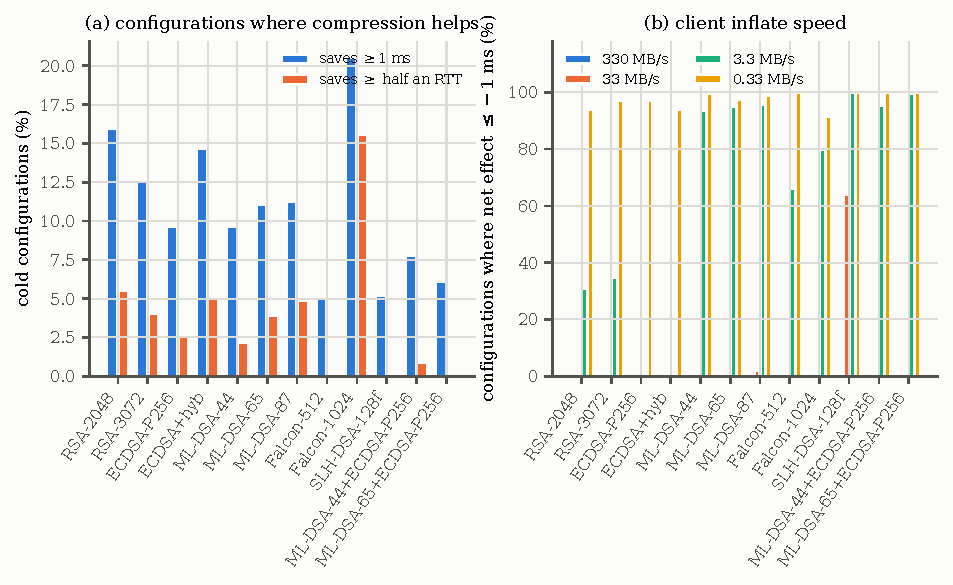
\includegraphics[width=\textwidth]{figures/fig_cc}
\caption{Effect of certificate compression.}
\label{fig:cc}
\end{figure}

\FloatBarrier
\section{Measured inputs and input checks}
\label{app:meas}
\Cref{tab:cpu} gives the per-operation medians on a performance core (Cortex-X925) and an efficiency core (Cortex-A725). \Cref{tab:certs} compares the DER sizes of the generated certificates with the sizes predicted from the ECDSA-calibrated metadata. \Cref{tab:comp_real} compares the zlib level-9 compression ratio of real chains with the model. Since the generated chains repeat names and extensions more often than public chains, classical chains compress better here than in the calibration set. \Cref{tab:tls} compares real TLS~1.3 handshake flights (OpenSSL~3.5.4, mTLS) with the calibrated model for the same certificates, and the loopback handshake time with the modeled handshake CPU time; CH denotes the ClientHello.

\begin{table}[!htbp]\centering\footnotesize
\caption{Per-operation CPU cost (ms).}
\label{tab:cpu}
\resizebox{0.92\textwidth}{!}{\begin{tabular}{@{}llrrrl@{}}
\toprule
Algorithm & Op. & X925 & A725 & A725/X925 & Implementation \\
\midrule
RSA-2048 & sign & 0.491 & 1.085 & 2.21 & OpenSSL 3.5.4 \\
RSA-2048 & verify & 0.0147 & 0.03163 & 2.15 & OpenSSL 3.5.4 \\
RSA-3072 & sign & 1.451 & 3.271 & 2.26 & OpenSSL 3.5.4 \\
RSA-3072 & verify & 0.0293 & 0.0648 & 2.21 & OpenSSL 3.5.4 \\
ECDSA-P256 & sign & 0.01446 & 0.02616 & 1.81 & OpenSSL 3.5.4 \\
ECDSA-P256 & verify & 0.04112 & 0.07835 & 1.91 & OpenSSL 3.5.4 \\
ML-DSA-44 & sign & 0.3594 & 0.753 & 2.10 & OpenSSL 3.5.4 \\
ML-DSA-44 & verify & 0.06804 & 0.1489 & 2.19 & OpenSSL 3.5.4 \\
ML-DSA-65 & sign & 0.586 & 1.225 & 2.09 & OpenSSL 3.5.4 \\
ML-DSA-65 & verify & 0.103 & 0.2289 & 2.22 & OpenSSL 3.5.4 \\
ML-DSA-87 & sign & 0.6691 & 1.438 & 2.15 & OpenSSL 3.5.4 \\
ML-DSA-87 & verify & 0.1589 & 0.3594 & 2.26 & OpenSSL 3.5.4 \\
Falcon-512 & sign & 0.1045 & 0.2057 & 1.97 & liboqs 0.14.0 \\
Falcon-512 & verify & 0.01755 & 0.0311 & 1.77 & liboqs 0.14.0 \\
Falcon-1024 & sign & 0.2114 & 0.4026 & 1.90 & liboqs 0.14.0 \\
Falcon-1024 & verify & 0.03098 & 0.05949 & 1.92 & liboqs 0.14.0 \\
SLH-DSA-128s & sign & 170.8 & 259.6 & 1.52 & OpenSSL 3.5.4 \\
SLH-DSA-128s & verify & 0.1614 & 0.2604 & 1.61 & OpenSSL 3.5.4 \\
SLH-DSA-128f & sign & 8.2 & 13.08 & 1.60 & OpenSSL 3.5.4 \\
SLH-DSA-128f & verify & 0.5058 & 0.7719 & 1.53 & OpenSSL 3.5.4 \\
\midrule
ECDHE-P256 & gen & 0.00845 & 0.01721 & 2.04 & OpenSSL 3.5.4 \\
ECDHE-P256 & derive & 0.03406 & 0.06565 & 1.93 & OpenSSL 3.5.4 \\
ECDHE-P256 & server & 0.04251 & 0.08286 & 1.95 & OpenSSL 3.5.4 \\
X25519 & gen & 0.01326 & 0.03127 & 2.36 & OpenSSL 3.5.4 \\
X25519 & derive & 0.0227 & 0.04522 & 1.99 & OpenSSL 3.5.4 \\
X25519 & server & 0.03596 & 0.07649 & 2.13 & OpenSSL 3.5.4 \\
X25519MLKEM768 & gen & 0.0311 & 0.07323 & 2.35 & OpenSSL 3.5.4 \\
X25519MLKEM768 & derive & 0.03734 & 0.08021 & 2.15 & OpenSSL 3.5.4 \\
X25519MLKEM768 & server & 0.04516 & 0.09852 & 2.18 & OpenSSL 3.5.4 \\
ML-KEM-768 & gen & 0.01784 & 0.04196 & 2.35 & OpenSSL 3.5.4 \\
ML-KEM-768 & derive & 0.01464 & 0.03499 & 2.39 & OpenSSL 3.5.4 \\
ML-KEM-768 & server & 0.0092 & 0.02203 & 2.40 & OpenSSL 3.5.4 \\
ML-KEM-1024 & gen & 0.02664 & 0.06338 & 2.38 & OpenSSL 3.5.4 \\
ML-KEM-1024 & derive & 0.01898 & 0.0458 & 2.41 & OpenSSL 3.5.4 \\
ML-KEM-1024 & server & 0.01183 & 0.02885 & 2.44 & OpenSSL 3.5.4 \\
\bottomrule
\end{tabular}}
\end{table}

\begin{table}[!htbp]\centering\small
\caption{Generated certificate sizes (bytes).}
\label{tab:certs}
\resizebox{\textwidth}{!}{\begin{tabular}{@{}lrrrrrr@{}}
\toprule
Algorithm & Leaf DER & CA DER & Metadata (leaf/CA) & Predicted leaf & Predicted CA & Max error (\%) \\
\midrule
RSA-2048 & 1416 & 1227 & 862/673 & 1408 & 1217 & 0.81 \\
RSA-3072 & 1672 & 1483 & 862/673 & 1664 & 1473 & 0.67 \\
ECDSA-P256 & 1021 & 830 & 854/663 & 1021 & 830 & 0.00 \\
ML-DSA-44 & 4616 & 4427 & 858/669 & 4612 & 4421 & 0.14 \\
ML-DSA-65 & 6145 & 5956 & 858/669 & 6141 & 5950 & 0.10 \\
ML-DSA-87 & 8103 & 7914 & 858/669 & 8099 & 7908 & 0.08 \\
SLH-DSA-128s & 8768 & 8579 & 854/665 & 8768 & 8577 & 0.02 \\
SLH-DSA-128f & 18000 & 17811 & 854/665 & 18000 & 17809 & 0.01 \\
\bottomrule
\end{tabular}}
\end{table}

\begin{table}[!htbp]\centering\small
\caption{Compression ratio of real chains.}
\label{tab:comp_real}
\resizebox{\textwidth}{!}{\begin{tabular}{@{}lrrrrrrrr@{}}
\toprule
Algorithm & \multicolumn{2}{c}{$d=1$} & \multicolumn{2}{c}{$d=2$} & \multicolumn{2}{c}{$d=3$} & \multicolumn{2}{c}{$d=4$} \\
\cmidrule(lr){2-3} \cmidrule(lr){4-5} \cmidrule(lr){6-7} \cmidrule(lr){8-9}
 & zlib-9 & model & zlib-9 & model & zlib-9 & model & zlib-9 & model \\
\midrule
RSA-2048 & 0.76 & 0.81 & 0.67 & 0.77 & 0.61 & 0.75 & 0.58 & 0.75 \\
RSA-3072 & 0.80 & 0.83 & 0.73 & 0.81 & 0.68 & 0.80 & 0.65 & 0.79 \\
ECDSA-P256 & 0.64 & 0.73 & 0.53 & 0.67 & 0.44 & 0.65 & 0.40 & 0.64 \\
ML-DSA-44 & 0.93 & 0.94 & 0.91 & 0.93 & 0.89 & 0.93 & 0.88 & 0.93 \\
ML-DSA-65 & 0.95 & 0.95 & 0.93 & 0.95 & 0.92 & 0.95 & 0.92 & 0.95 \\
ML-DSA-87 & 0.96 & 0.97 & 0.95 & 0.96 & 0.94 & 0.96 & 0.94 & 0.96 \\
SLH-DSA-128s & 0.96 & 0.97 & 0.95 & 0.96 & 0.95 & 0.96 & 0.94 & 0.96 \\
SLH-DSA-128f & 0.98 & 0.98 & 0.98 & 0.98 & 0.98 & 0.98 & 0.97 & 0.98 \\
\bottomrule
\end{tabular}}
\end{table}

\begin{table}[!htbp]\centering\small
\caption{Real TLS~1.3 handshake flights (bytes).}
\label{tab:tls}
\resizebox{\textwidth}{!}{\begin{tabular}{@{}lrrrrrrrr@{}}
\toprule
Suite (mutual TLS) & $d$ & CH & Server flight & Client flight & Model total & Error (\%) & Loopback (ms) & Model CPU (ms) \\
\midrule
RSA-2048 & 1 & 323 & 2075 & 1812 & 4202 & $-$0.19 & 2.00 & 1.13 \\
RSA-2048 & 4 & 323 & 5771 & 5508 & 11594 & $-$0.07 & 2.07 & 1.21 \\
RSA-3072 & 1 & 323 & 2459 & 2196 & 4970 & $-$0.16 & 4.21 & 3.10 \\
RSA-3072 & 4 & 323 & 6923 & 6660 & 13898 & $-$0.06 & 4.38 & 3.28 \\
ECDSA-P256 (baseline) & 1 & 290 & 1460 & 1231 & 2974 & $-$0.23 & 0.74 & 0.27 \\
ECDSA-P256 (baseline) & 4 & 290 & 3969 & 3737 & 7992 & $-$0.05 & 0.85 & 0.51 \\
ECDSA-P256 + hybrid KEM & 1 & 1466 & 2548 & 1231 & 5246 & 0.02 & 0.59 & 0.31 \\
ECDSA-P256 + hybrid KEM & 4 & 1466 & 5057 & 3737 & 10264 & 0.04 & 0.82 & 0.55 \\
ML-DSA-44 & 1 & 1434 & 8462 & 7176 & 17072 & 0.00 & 0.97 & 1.03 \\
ML-DSA-44 & 4 & 1434 & 21780 & 20494 & 43708 & 0.00 & 1.51 & 1.44 \\
ML-DSA-65 & 1 & 1434 & 10880 & 9594 & 21908 & 0.00 & 1.89 & 1.63 \\
ML-DSA-65 & 4 & 1434 & 28785 & 27499 & 57718 & 0.00 & 2.23 & 2.24 \\
ML-DSA-87 & 1 & 1818 & 14636 & 12870 & 29324 & 0.00 & 2.31 & 2.03 \\
ML-DSA-87 & 4 & 1818 & 38415 & 36649 & 76882 & 0.00 & 2.36 & 2.98 \\
\bottomrule
\end{tabular}}
\end{table}

\FloatBarrier
\section{Internet check, application objects, sensitivity, residuals and status}
\label{app:more}
\Cref{tab:internet} reports real-Internet handshakes with X25519 and X25519\allowbreak{}MLKEM768 over 100 interleaved rounds per server: median times, the paired difference with its bootstrap 95\% confidence interval and the extra bytes. \Cref{tab:app} compares real signed application objects with the model: the JWS client assertion and access token, the DPoP proof and the XMLDSig over a pacs.008 document with the signer certificate in \texttt{KeyInfo}. \Cref{tab:sobol} lists the largest first- and second-order variance-based indices of log latency and of the log post-quantum (PQ) factor over the full factorial wired designs. \Cref{tab:uncertainty} summarizes the 4\,000 draws of \cref{M-sec:rq5} by median and 5th and 95th percentiles; probabilities appear in the median column.

\begin{table}[!htbp]\centering\small
\caption{Real-Internet handshakes.}
\label{tab:internet}
\resizebox{\textwidth}{!}{\begin{tabular}{@{}lrrrrr@{}}
\toprule
Server & RTT (ms) & X25519 (ms) & X25519MLKEM768 (ms) & Paired difference (ms) & Extra bytes out/in \\
\midrule
cloudflare.com & 30 & 35.4 & 37.0 & 2.9 [1.2, 4.4] & 1176/1088 \\
www.google.com & 34 & 62.9 & 65.9 & 2.5 [0.1, 5.7] & 1176/1088 \\
\bottomrule
\end{tabular}}
\end{table}

\begin{table}[!htbp]\centering\small
\caption{Real signed application objects (bytes).}
\label{tab:app}
\resizebox{\textwidth}{!}{\begin{tabular}{@{}lrrrrrrrr@{}}
\toprule
Algorithm & \multicolumn{2}{c}{Client assertion} & \multicolumn{2}{c}{Access token} & \multicolumn{2}{c}{DPoP proof} & \multicolumn{2}{c}{XMLDSig} \\
\cmidrule(lr){2-3}\cmidrule(lr){4-5}\cmidrule(lr){6-7}\cmidrule(l){8-9}
 & real & model & real & model & real & model & real & model \\
\midrule
ECDSA-P256 & 381 & 536 & 549 & 796 & 518 & 732 & 2268 & 2270 \\
RSA-2048 & 637 & 782 & 805 & 1042 & 1104 & 1342 & 3055 & 3034 \\
ML-DSA-44 & 3527 & 3667 & 3695 & 3927 & 5883 & 6081 & 10182 & 10190 \\
ML-DSA-65 & 4712 & 4852 & 4880 & 5112 & 8206 & 8403 & 13406 & 13414 \\
ML-DSA-87 & 6470 & 6610 & 6638 & 6870 & 11101 & 11298 & 17774 & 17782 \\
SLH-DSA-128s & 10786 & 10915 & 10954 & 11175 & 10877 & 11053 & 22969 & 22978 \\
SLH-DSA-128f & 23095 & 23224 & 23263 & 23484 & 23186 & 23362 & 47585 & 47598 \\
\bottomrule
\end{tabular}}
\end{table}

\begin{table}[!htbp]\centering\small
\caption{Global sensitivity indices.}
\label{tab:sobol}
\resizebox{\textwidth}{!}{\begin{tabular}{@{}lp{0.68\textwidth}@{}}
\toprule
Response & Largest first- and second-order indices \\
\midrule
log latency, wired & RTT (0.59), suite (0.28), suite $\times$ RTT (0.04), protocol (0.03), MTU (0.02) \\
log PQ factor, wired, all PQ suites & suite (0.68), RTT (0.12), suite $\times$ RTT (0.09), MTU (0.02), protocol (0.01) \\
log PQ factor, wired, ML-DSA and Falcon & RTT (0.20), MTU (0.18), suite (0.16), penalty (0.09), protocol (0.06) \\
\bottomrule
\end{tabular}}
\end{table}

\begin{table}[!htbp]\centering\small
\caption{Assumption-based uncertainty, SWIFT~MX.}
\label{tab:uncertainty}
\begin{tabular}{@{}lrrr@{}}\toprule
Metric & Median & 5th pct. & 95th pct. \\\midrule
ML-DSA-65 latency (ms) & 179.6 & 115.1 & 238.5 \\
ML-DSA-65 factor over baseline & 1.46 & 1.19 & 1.72 \\
Falcon-512 factor & 1.05 & 1.01 & 1.23 \\
SLH-DSA-128f factor & 3.34 & 2.31 & 6.21 \\
SLH-DSA-128s factor & 25.6 & 8.2 & 79.4 \\
ML-DSA-65 $\bar{\Delta}_d$ (ms) & 20.5 & 3.5 & 27.9 \\
$\Pr(O>T_\mathrm{cpu})$ & 0.91 & \multicolumn{2}{c}{--} \\
$\Pr$(Falcon-512 $<$ ML-DSA-65 $<$ SLH-DSA-128f) & 1.00 & \multicolumn{2}{c}{--} \\
\bottomrule\end{tabular}
\end{table}

\Cref{tab:ablation} gives the contribution of each stack mechanism on the 226 validation configurations, and \cref{tab:priors} lists the prior distributions of the uncertainty analysis of \cref{M-sec:rq5} (script \texttt{uncertainty.py}, seed 1; \texttt{--pi0} fixes $\pi=0$).

\begin{table}[!htbp]\centering\small
\caption{Contribution of each stack mechanism: excess-latency prediction error on the 226 validation configurations (model minus measurement). Nothing is fitted (\texttt{ablation\_stack.py}).}
\label{tab:ablation}
\resizebox{\textwidth}{!}{\begin{tabular}{@{}lrrrr@{}}
\toprule
Model & MAE (ms) & Bias (ms) & \shortstack[r]{Maximum\\error (ms)} & \shortstack[r]{Configurations\\above 0.4\,RTT} \\
\midrule
Idealized (no mechanism) & 4.70 & $-3.5$ & 97.1 & 21 \\
Window validation only & 3.34 & $-2.0$ & 95.4 & 12 \\
OpenSSL write boundaries only & 3.15 & $-1.8$ & 95.3 & 15 \\
Both (model of this paper) & 1.65 & $+0.1$ & 5.4 & 4 \\
\bottomrule
\end{tabular}}
\end{table}

\begin{table}[!htbp]\centering\small
\caption{Prior distributions of the uncertainty analysis (4\,000 draws, seed 1). The inputs are drawn independently, except that the metadata of leaf and CA certificates share one quantile and so move together. The priors are assumptions, not fitted distributions.}
\label{tab:priors}
\begin{tabularx}{\textwidth}{@{}>{\raggedright\arraybackslash}p{0.22\textwidth}>{\raggedright\arraybackslash}p{0.34\textwidth}>{\raggedright\arraybackslash}X@{}}
\toprule
Input & Distribution & Basis \\
\midrule
Leaf certificate metadata & uniform, 600--1\,400\,bytes & range around the calibrated 900\,bytes \\
CA certificate metadata & uniform, 350--800\,bytes (same quantile as the leaf) & range around the calibrated 520\,bytes \\
CPU scale & log-uniform, 1--16 & 1 measured X925, 4 measured x86, 16 assumed \\
Middlebox delay $\pi$ & uniform, 0--24\,ms & assumption; the HAProxy measurements support 0 \\
Segment threshold $\theta$ & uniform on the integers 2--16 & assumption \\
Initial window & 10, 32, 64 segments with probabilities 0.6, 0.3, 0.1 & RFC~6928 default and larger production windows \\
\bottomrule
\end{tabularx}
\end{table}

\Cref{tab:cpux86} compares the primitive costs on the critical path for the Cortex-X925 (simulator default), the Cortex-A725 and one core of the Intel Core i7-5600U (2.5\,GHz, AVX2, turbo disabled), with the same method. \Cref{tab:residuals} and \cref{fig:residuals} break down the stack-model error (model minus measurement) by configuration group. The 95\% interval of the MAE uses 2\,000 bootstrap resamples of the configurations. The core grid is the identification set (100\Mbits, initial window of 10 segments). The off-grid set comes from a later campaign on the same day (UTC 07:51--08:35 for the core grid and 09:07--09:17 off-grid); no model parameter was fitted to it. All rows use Reno, no loss, mTLS and the direct path.

\begin{table}[!htbp]\centering\small
\caption{Primitive cost on three cores (ms).}
\label{tab:cpux86}
\begin{tabular}{@{}llrrrr@{}}
\toprule
Primitive & Operation & X925 (ms) & A725 (ms) & x86 (ms) & x86/X925 \\
\midrule
RSA-2048 & sign & 0.491 & 1.09 & 0.835 & 1.7 \\
RSA-2048 & verify & 0.0147 & 0.0316 & 0.0334 & 2.3 \\
ECDSA-P256 & sign & 0.0145 & 0.0262 & 0.0402 & 2.8 \\
ECDSA-P256 & verify & 0.0411 & 0.0783 & 0.102 & 2.5 \\
ML-DSA-44 & sign & 0.359 & 0.753 & 1.05 & 2.9 \\
ML-DSA-44 & verify & 0.068 & 0.149 & 0.213 & 3.1 \\
ML-DSA-65 & sign & 0.586 & 1.22 & 1.72 & 2.9 \\
ML-DSA-65 & verify & 0.103 & 0.229 & 0.326 & 3.2 \\
ML-DSA-87 & sign & 0.669 & 1.44 & 1.95 & 2.9 \\
ML-DSA-87 & verify & 0.159 & 0.359 & 0.508 & 3.2 \\
Falcon-512 & sign & 0.105 & 0.206 & 0.361 & 3.4 \\
Falcon-512 & verify & 0.0176 & 0.0311 & 0.065 & 3.7 \\
SLH-DSA-128s & sign & 171 & 260 & 1\,320 & 7.7 \\
SLH-DSA-128s & verify & 0.161 & 0.26 & 1.3 & 8.1 \\
SLH-DSA-128f & sign & 8.2 & 13.1 & 63.1 & 7.7 \\
SLH-DSA-128f & verify & 0.506 & 0.772 & 3.79 & 7.5 \\
X25519 & key generation & 0.0133 & 0.0313 & 0.0513 & 3.9 \\
X25519 & derive & 0.0227 & 0.0452 & 0.0509 & 2.2 \\
ML-KEM-768 & key generation & 0.0178 & 0.042 & 0.0641 & 3.6 \\
ML-KEM-768 & encapsulate & 0.0092 & 0.022 & 0.04 & 4.3 \\
ML-KEM-768 & decapsulate & 0.0146 & 0.035 & 0.0608 & 4.2 \\
\bottomrule
\end{tabular}
\end{table}

\begin{table}[!htbp]\centering\small
\caption{Stack-model error by configuration group.}
\label{tab:residuals}
\resizebox{\textwidth}{!}{\begin{tabular}{@{}llrrrrr@{}}
\toprule
Group & Value & $n$ & MAE (ms) & RMSE (ms) & MAE / mean excess (\%) & MAE 95\% interval (ms) \\
\midrule
 & all configurations & 226 & 1.65 & 2.16 & 1.2 & 1.48--1.83 \\
\midrule
 & core grid (100\,Mbit/s, initial window 10) & 82 & 0.96 & 1.34 & 0.6 & 0.77--1.18 \\
 & off-grid (later campaign) & 144 & 2.04 & 2.51 & 1.8 & 1.81--2.28 \\
\midrule
RTT (ms) & 5 & 24 & 0.95 & 1.31 & 4.9 & 0.63--1.33 \\
RTT (ms) & 30 & 178 & 1.84 & 2.34 & 1.6 & 1.63--2.05 \\
RTT (ms) & 100 & 24 & 0.92 & 1.30 & 0.2 & 0.57--1.31 \\
\midrule
MTU (bytes) & 1280 & 58 & 1.87 & 2.39 & 1.5 & 1.50--2.26 \\
MTU (bytes) & 1500 & 120 & 1.33 & 1.83 & 0.9 & 1.12--1.57 \\
MTU (bytes) & 9000 & 48 & 2.17 & 2.61 & 2.1 & 1.77--2.58 \\
\midrule
initial window & 10 & 154 & 1.32 & 1.80 & 0.9 & 1.13--1.52 \\
initial window & 32 & 72 & 2.35 & 2.79 & 2.2 & 2.01--2.70 \\
\midrule
chain depth & 1 & 60 & 1.72 & 2.21 & 1.4 & 1.36--2.06 \\
chain depth & 2 & 58 & 1.58 & 2.00 & 1.2 & 1.28--1.89 \\
chain depth & 3 & 54 & 1.59 & 2.17 & 1.1 & 1.21--1.98 \\
chain depth & 4 & 54 & 1.70 & 2.27 & 1.2 & 1.33--2.13 \\
\midrule
suite & ECDSA-P256 & 63 & 1.48 & 1.89 & 1.4 & 1.19--1.77 \\
suite & ECDSA + hybrid KEM & 15 & 0.64 & 0.64 & 0.5 & 0.60--0.67 \\
suite & ML-DSA-44 & 12 & 0.72 & 0.90 & 0.4 & 0.43--1.03 \\
suite & ML-DSA-65 & 62 & 1.89 & 2.38 & 1.4 & 1.54--2.25 \\
suite & ML-DSA-87 & 62 & 2.14 & 2.67 & 1.4 & 1.75--2.54 \\
suite & RSA-2048 & 12 & 0.95 & 1.38 & 0.7 & 0.40--1.51 \\
\bottomrule
\end{tabular}}
\end{table}

\begin{figure}[!htbp]\centering
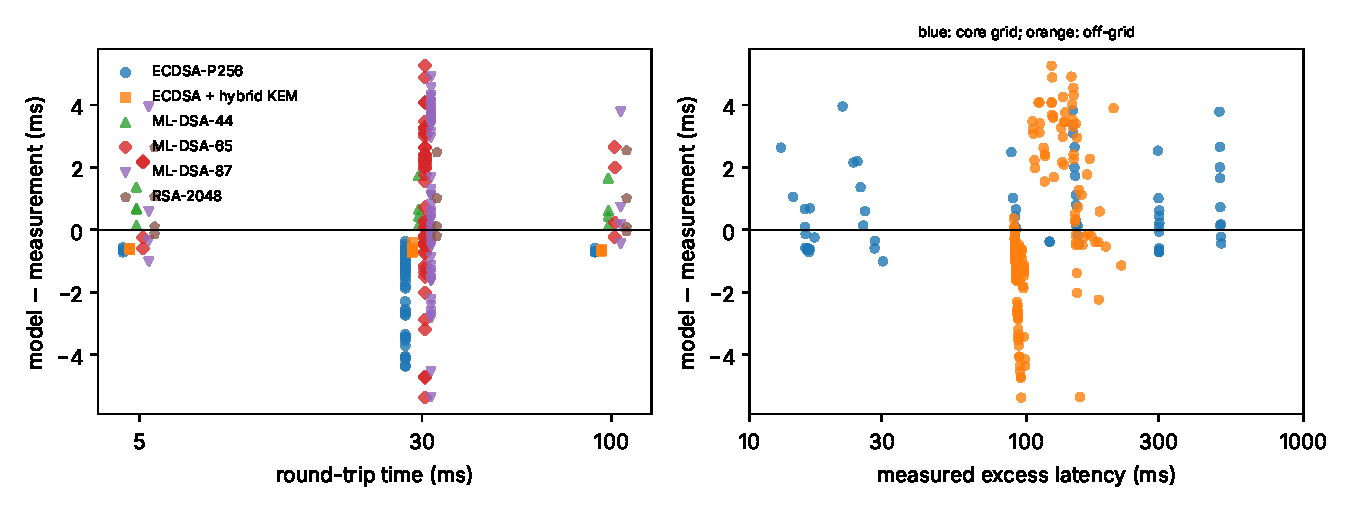
\includegraphics[width=\textwidth]{figures/fig_residuals}
\caption{Residuals of the stack model.}
\label{fig:residuals}
\end{figure}

In \cref{fig:residuals}, the left panel plots the residuals of the 82 core-grid and 144 off-grid configurations against the RTT by suite, and the right panel plots them against the measured excess latency. \Cref{tab:variants} evaluates the stack model under other TCP settings at 100\Mbits. Its columns give the MAE of the stack model and of the idealized model, the bias and maximum error of the stack model, the number of configurations above 0.4\,RTT (stack / idealized) and the difference $\Delta$ of measured excess latency against the Reno, quick-acknowledgment, no-timestamp run of the same configuration. CUBIC covers 5, 30 and 100\ms RTT, MTUs of 1\,280, 1\,500 and 9\,000\,bytes and initial windows of 10 and 32. The other rows use MTUs of 1\,280 and 1\,500\,bytes, an initial window of 10 and three suites. The model does not represent BBR; the BBR row marks the limit of the model.

\begin{table}[!htbp]\centering\small
\caption{Stack model under other TCP settings.}
\label{tab:variants}
\resizebox{\textwidth}{!}{\begin{tabular}{@{}lrrrrrrrrr@{}}
\toprule
Variant & $n$ & MAE (ms) & idealized MAE (ms) & bias (ms) & max (ms) & off $>0.4$ RTT (stack / idealized) & pairs & median $\Delta$ (ms) & max $|\Delta|$ (ms) \\
\midrule
CUBIC, quick ACK & 216 & 1.19 & 5.43 & +0.61 & 5.1 & 12 / 18 & 42 & +0.10 & 1.4 \\
Reno, delayed ACK & 72 & 1.26 & 11.04 & +0.48 & 3.8 & 5 / 11 & 42 & +0.14 & 0.7 \\
Reno, quick ACK, timestamps & 72 & 1.32 & 11.04 & +0.55 & 4.3 & 6 / 11 & 42 & +0.15 & 1.5 \\
Reno, delayed ACK, timestamps & 72 & 1.23 & 11.10 & +0.48 & 3.5 & 8 / 12 & 42 & +0.12 & 1.5 \\
BBR, quick ACK (exploratory) & 8 & 3.51 & 3.54 & -3.23 & 21.8 & 0 / 0 & 8 & +0.13 & 24.4 \\
\bottomrule
\end{tabular}}
\end{table}

\Cref{tab:status} records the standardization status of each scheme on 31 October 2026, read from csrc.nist.gov and datatracker.ietf.org on that date (the draft of the pure ML-KEM groups~\cite{tlsmlkem} on 2 November 2026), and the measured components. TLS marks a run through a real TLS~1.3 handshake on the testbed. CPU marks a measured per-operation cost (\cref{tab:cpu,tab:cpux86}). Sizes marks certificate and signature sizes from real generated or published objects. Unmeasured quantities are modeled. Standardization status does not indicate deployment readiness, and the table does not assess library or HSM support.

\begin{table}[!htbp]\centering\footnotesize
\caption{Standardization status and measured components.}
\label{tab:status}
\resizebox{\textwidth}{!}{\begin{tabular}{@{}>{\raggedright\arraybackslash}p{0.15\textwidth}>{\raggedright\arraybackslash}p{0.17\textwidth}>{\raggedright\arraybackslash}p{0.17\textwidth}>{\raggedright\arraybackslash}p{0.22\textwidth}>{\raggedright\arraybackslash}p{0.05\textwidth}>{\raggedright\arraybackslash}p{0.05\textwidth}>{\raggedright\arraybackslash}p{0.06\textwidth}@{}}
\toprule
Scheme & NIST standard & X.509 profile (IETF) & TLS~1.3 specification & TLS & CPU & Sizes \\
\midrule
RSA-2048, ECDSA-P256 & FIPS 186-5 & RFC 5280 & RFC 9846 & yes & yes & yes \\
ML-KEM-768/1024; X25519\allowbreak{}MLKEM768 & FIPS 203 (13 Aug 2024) & -- & X25519\allowbreak{}MLKEM768: RFC 10024 (Aug 2026); pure ML-KEM groups: not assessed & yes & yes & yes \\
ML-DSA-44/65/87 & FIPS 204 (13 Aug 2024) & RFC 9881 (Oct 2025) & draft-ietf-tls-mldsa-06, RFC Editor queue, Informational & yes & yes & yes \\
SLH-DSA-128s/128f & FIPS 205 (13 Aug 2024) & RFC 9909 (Dec 2025) & no code points in OpenSSL~3.5 & no & yes & yes (certificates) \\
Falcon-512 (FN-DSA) & FIPS 206 in development (round-3 parameters used here) & draft-ietf-lamps-fn-dsa-certificates-00 (May 2026) & none & no & yes (liboqs) & sizes of the specification \\
Composite ML-DSA + ECDSA & -- & draft-ietf-lamps-pq-composite-sigs-19, RFC Editor queue & none & no & sum & sizes of the sum \\
\bottomrule
\end{tabular}}
\end{table}

\FloatBarrier

\section{Session tickets and server CPU}
\label{app:extra}
\Cref{tab:ticket} compares a full transaction that also issues a TLS~1.3 session ticket with the ticketless transaction of the main campaign. \Cref{tab:srvcpu} compares the CPU per transaction of an event-driven server with the primitive costs of the model.

\emph{A model test.} The slow configurations are ECDSA-P256 at depth 3 and ML-DSA-44 and -65 at depth 1, all at an MTU of 1\,500 bytes and at RTTs of 30 and 100\ms; ECDSA-P256 and ML-DSA-87 at depth 1, the 1\,280-byte runs and the other depths are within about 2\ms. We gave the model an option for a cold flow whose server issues a ticket of the size used for resumed flows (\texttt{Model(full\_ticket=True)}), either joined with the first response or written on the client's Finished (\texttt{analyze\_fullticket.py}, nothing fitted). Neither placement reproduces the slowdown: in the six slow configurations the model changes by $+0.1$ to $+0.5$\ms while the measurement changes by $+14.9$ to $+50.8$\ms, and the mean absolute error over the 40 configurations is 5.96\ms without a ticket, 5.87\ms with the ticket joined and 5.83\ms with it written on the Finished (six configurations off by more than 5\ms in each case). A ticket as an extra write does not explain the half round trip; its cause is not established, so the model keeps no ticket mode for full handshakes.

\begin{table}[!htbp]\centering\small
\caption{A full transaction that also issues a session ticket against the ticketless one of the main campaign (excess latency over the unshaped run, ms; same suite, chain depth, RTT, MTU, initial window of 10, 100\Mbits, 302/222-byte transaction, Reno with quick acknowledgments). The model has no mode for a full handshake with a ticket. In 6 of the 40 configurations that have a ticketless reference, the transaction with a ticket was slower by half a round trip (median 0.51 RTT); the median difference over all is 0.6\ms.}
\label{tab:ticket}
\resizebox{\textwidth}{!}{\begin{tabular}{@{}lrrrrrr@{}}
\toprule
Suite & depth & MTU & \multicolumn{3}{c}{ticket minus no ticket (ms) at RTT} & in RTT \\
\cmidrule(lr){4-6}
 & & & 5\,ms & 30\,ms & 100\,ms & (30, 100\,ms) \\
\midrule
ECDSA-P256 & 1 & 1280 & -- & +0.2 & -- & +0.01 \\
ECDSA-P256 & 1 & 1500 & +0.2 & +0.3 & +0.4 & +0.01 \\
ECDSA-P256 & 3 & 1500 & +0.3 & +14.9 & +50.1 & +0.50 \\
ECDSA-P256 + hybrid KEM & 1 & 1280 & -- & +0.2 & -- & +0.01 \\
ECDSA-P256 + hybrid KEM & 1 & 1500 & +0.2 & +0.2 & +0.2 & +0.00 \\
ECDSA-P256 + hybrid KEM & 3 & 1500 & +0.3 & +0.3 & +0.4 & +0.01 \\
ML-DSA-44 & 1 & 1500 & +1.2 & +15.6 & +50.8 & +0.51 \\
ML-DSA-44 & 3 & 1500 & +0.8 & +0.9 & +0.9 & +0.02 \\
ML-DSA-65 & 1 & 1280 & -- & -0.1 & -- & -0.00 \\
ML-DSA-65 & 1 & 1500 & +0.5 & +15.8 & +50.8 & +0.52 \\
ML-DSA-65 & 3 & 1500 & +0.8 & +0.8 & +0.9 & +0.02 \\
ML-DSA-87 & 1 & 1280 & -- & +0.6 & -- & +0.02 \\
ML-DSA-87 & 1 & 1500 & +0.6 & +0.7 & +0.6 & +0.01 \\
ML-DSA-87 & 3 & 1500 & +0.9 & +0.9 & +1.0 & +0.02 \\
RSA-2048 & 1 & 1500 & +1.9 & +2.0 & +2.0 & +0.04 \\
RSA-2048 & 3 & 1500 & +0.3 & +0.2 & +0.3 & +0.00 \\
\bottomrule
\end{tabular}
}
\end{table}

\begin{table}[!htbp]\centering\small
\caption{CPU per transaction of an event-driven OpenSSL~3.5.4 server on one Cortex-X925 core (loopback, saturated by a multi-threaded load generator; user and system CPU of the server process over the measurement window divided by the transactions it completed; ms) against the sum of the primitive costs of the model for the same operations. Chain depth 2, or 1 for resumed.}
\label{tab:srvcpu}
\resizebox{\textwidth}{!}{\begin{tabular}{@{}lrrrrrrrrr@{}}
\toprule
Suite & \multicolumn{3}{c}{server auth, depth 2} & \multicolumn{3}{c}{mutual TLS, depth 2} & \multicolumn{3}{c}{resumed, mutual TLS} \\
\cmidrule(lr){2-4}\cmidrule(lr){5-7}\cmidrule(lr){8-10}
 & measured & primitives & ratio & measured & primitives & ratio & measured & primitives & ratio \\
\midrule
ECDSA-P256 & 0.137 & 0.050 & 2.7 & 0.323 & 0.174 & 1.9 & 0.182 & 0.036 & 5.0 \\
ECDSA-P256 + hybrid KEM & 0.165 & 0.060 & 2.8 & 0.350 & 0.183 & 1.9 & 0.211 & 0.045 & 4.7 \\
RSA-2048 & 0.631 & 0.533 & 1.2 & 0.739 & 0.578 & 1.3 & 0.193 & 0.043 & 4.5 \\
ML-DSA-44 & 0.480 & 0.369 & 1.3 & 0.755 & 0.573 & 1.3 & 0.175 & 0.009 & 19.1 \\
ML-DSA-65 & 0.722 & 0.595 & 1.2 & 1.105 & 0.904 & 1.2 & 0.182 & 0.009 & 19.8 \\
ML-DSA-87 & 0.838 & 0.681 & 1.2 & 1.399 & 1.157 & 1.2 & 0.198 & 0.012 & 16.7 \\
\bottomrule
\end{tabular}
}
\end{table}

\emph{Reading the ratio.} The difference between the measured CPU and the primitives is 0.09--0.24\ms in every row (0.15--0.19\ms for resumed handshakes), whereas the primitives range from 0.009\ms (resumed, post-quantum) to 1.16\ms (ML-DSA-87, mutual TLS). The measured CPU therefore contains a cost per connection that the primitive costs of the model do not include (accepting the connection, the record layer, hashing and key derivation of the transcript, ticket handling, the event loop). It is a small part of a post-quantum full handshake (ratio 1.2--1.3), a larger part of a classical one (1.9--2.8) and almost the whole of a resumed handshake (4.5--19.8, at 0.18--0.21\ms), which is why the ratio is large exactly where the primitives are cheap. We did not separate the components of this cost.

\FloatBarrier
\section{Application messages above one TLS record}
\label{app:records}
\emph{What the model assumes.} The model of the main text writes each application message, a request or a response, to the socket at once. The OpenSSL~3.5 library does so only for messages that fit in one TLS record. \texttt{SSL\_write()} splits a longer message into records of at most 16\,384\,bytes of plaintext and sends each record, with its 22\,bytes of framing, as a write of its own. With \texttt{TCP\_NODELAY}, the end of a record can leave a partial segment at once when the window permits, which is the write-boundary mechanism that \cref{M-sec:mech} establishes for handshake data. A message above 16\,KB therefore has more write boundaries than the model assumes. Handshake messages are not affected, since the model already accounts for their records and the 4\,096-byte buffer.

\emph{What was validated.} No validated transaction contains a message above one record: the requests and responses measured on the testbed are 302 and 222\,bytes, and 10.9 and 3.6\,KiB in the SWIFT-sized experiment. The write pattern of messages above one record is therefore not validated in this paper. The model has the option \texttt{Model(app\_records=True)} (\texttt{pqc\_sim.py}), which writes each message as one write per record. The option is off in every result of this paper.

\emph{Method.} We repeated the cold and warm grids of the main sweep with $\pi=0$ with the option on and compared the outputs with the reference model: thirteen suites, six profiles, chain depths 1--4 for cold connections (one state for warm ones), six bit rates, five RTTs and three MTUs, with a CPU scale of 1 and a window of 10 segments, so that each suite has 2\,160 cold and 540 warm rows. A flow is affected when at least one of its messages exceeds 16\,KB; the write list of an unaffected flow is the same with and without the option, and so is its latency. The script is \texttt{app\_records\_effect.py}, and its outputs are \texttt{app\_records\_effect.csv} and \texttt{app\_records\_examples.csv}.

\emph{Results.} The option changes the write list of 76 of the 312 cold flows and of 19 of the 78 warm flows. The affected cold flows belong to the ML-DSA, Falcon-1024, SLH-DSA and composite suites; no flow of the RSA, ECDSA, hybrid or Falcon-512 suites is affected (\cref{tab:records}). In a warm row the largest change is 0.1\,ms. In a cold row it is at most 1.2\,ms for every suite except the two SLH-DSA suites, in which 143 of 4\,320 rows change by more than 0.5\,ms, by up to 100\,ms. The share $\phi$ of rows in which the size-dependent overhead exceeds the modeled primitive time is the same with and without the option, to the precision of \cref{tab:records}. In the reference scenario of \cref{M-sec:results} (SWIFT~MX, 100\Mbits, 30\ms RTT, MTU of 1\,500\,bytes), only SLH-DSA-128f at depth~1 changes, from 226.6 to 252.7\ms; the increase from depth 1 to 4 for this suite becomes 38.9\ms instead of 64.9\ms (\cref{M-tab:master,tab:sens}). The entries of the other suites, including the ML-DSA-65 increase of 60.0\ms and the share of 75.6\%, stay the same to 0.1\ms.

\emph{Reading of the results.} The conclusions on ML-DSA, Falcon and the classical suites do not depend on this simplification. The SLH-DSA entries that involve messages above 16\,KB, that is, the signed objects of the larger profiles, may differ by up to the amounts of \cref{tab:records}; their direction is not established. These suites cannot run in OpenSSL~3.5 TLS (\cref{M-tab:evidence}), so the entries are not measured either way. A test of the record-write pattern would need messages above 16\,KB on the testbed.

\begin{table}[!htbp]\centering\small
\caption{Effect of writing application messages as one write per TLS record on the model outputs (cold connections, main-sweep grid with $\pi=0$, CPU scale 1; \texttt{app\_records\_effect.py}). Flows: affected flows, of the 24 combinations of profile and chain depth of each suite. Rows $>0.5$\,ms: rows whose latency changes by more than 0.5\,ms, of the 2\,160 combinations of bit rate, RTT and MTU of each suite. Largest: largest absolute change. $\phi$ and $\phi$ with: share of rows with $O>T_\mathrm{cpu}$ (\cref{M-eq:share}) without and with the option. The RSA-2048, RSA-3072, ECDSA-P256, ECDSA-P256 + hybrid KEM and Falcon-512 suites have no affected flow.}
\label{tab:records}
\resizebox{\textwidth}{!}{\begin{tabular}{@{}lrrrrr@{}}
\toprule
Suite & Flows & Rows $>0.5$\,ms & Largest (ms) & $\phi$ (\%) & $\phi$ with (\%) \\
\midrule
ML-DSA-44 & 4 & 0 & 0.0 & 70.6 & 70.6 \\
ML-DSA-65 & 8 & 0 & 0.0 & 75.6 & 75.6 \\
ML-DSA-87 & 12 & 2 & 1.2 & 79.4 & 79.4 \\
Falcon-1024 & 4 & 0 & 0.0 & 72.7 & 72.7 \\
SLH-DSA-128s & 16 & 27 & 99.7 & 0.3 & 0.3 \\
SLH-DSA-128f & 20 & 116 & 99.8 & 70.6 & 70.6 \\
ML-DSA-44+ECDSA-P256 & 4 & 0 & 0.0 & 69.0 & 69.0 \\
ML-DSA-65+ECDSA-P256 & 8 & 0 & 0.0 & 73.2 & 73.2 \\
\bottomrule
\end{tabular}}
\end{table}

%% References (generated with elsarticle-num and included here)

\begin{thebibliography}{1}
\bibitem{tlsmlkem}
D.~Connolly, {ML-KEM} post-quantum key agreement for {TLS} 1.3, Internet-Draft
  draft-ietf-tls-mlkem-11 (in the RFC Editor queue, intended Informational),
  {IETF}, accessed 2 November 2026 (2026).
\end{thebibliography}

\end{document}
